%&plurals_event
% %PRECOMPILE COMMAND pdftex -ini -jobname="plurals_event_chap_34" "&pdflatex" mylatexformat.ltx plurals_event_chap_34.tex
% \documentclass[english]{article}
% \usepackage[T1]{fontenc}
% \usepackage[latin1]{inputenc}
% \usepackage[sort]{natbib}
% \usepackage{stdprmbl}

% \usepackage{parskip}

% \lingset{interpartskip = -5pt}
% \lingset{aboveexskip = 3pt,belowexskip = 3pt, belowpreambleskip = -3pt}

% \newcommand{\ag}{\textsc{Agent}}
% \newcommand{\thm}{\textsc{Theme}}
% \newcommand{\goal}{\textsc{Goal}}

\endofdump

\definecolor{darkred}{rgb}{0.4,0,0}
\newcommand{\scale}{1}

\title{Plurals and events (chap. 7) : First-order and second-order quantification}
\author{Keny Chatain}

\begin{document}
\maketitle

Last chapter spelled out the basic ingredients of the syntax/semantics interface focusing on thematic roles and the position of quantification. In this chapter, Schein spells out a little bit more the interpretation of quantifiers ; some of the assumptions made in the previous chapter are revised.


\section{First-order quantification: \emph{every}, \emph{some\textsubscript{sg}}, \emph{no\textsubscript{sg}}}
%
His theory comports two types of quantifiers: first-order quantifiers (i.e. quantifiers over singularities) and second-order quantifiers (i.e. quantifiers over pluralities). 

\paragraph{Sub-events.} Last chapter, we saw evidence that \emph{every} must be associated with quantification over sub-events to account for \cnextxa.

\pex
\a
Gracefully, every quarterback pushed the pram up the hill.
\a
$\exists E,\ \text{gracefully}(e) \wedge \forall x\in\dbb{quarterback}, \exists E,\ \textsc{Agent}(E) = x \wedge \text{pushed-the-pram-up-the-hill}(E)$ 
\xe
%
This logical formula in \clastxb is adequate to capture the meaning of \clastxa. (Remember that an existential quantifier over events that use the same variable as a previous existential quantifier is interpreted as quantifying over a subpart of it) It also captures

It also captures distributivity since each element in the restrictor is associated with its own sub-event:

\pex
\a
Gracefully, every boy ate a crisp.
\a
$\exists E,\ \text{gracefully}(e) \wedge \forall x\in\dbb{quarterback}, \exists E,\ \textsc{Agent}(E) = x \wedge \text{ate}(E) \wedge \exists y\in\dbb{crisp}, \textsc{Theme}(E) = y$ 
\xe
%
More generally, one would like to say that every (first-order) quantifier is associated with such an existential. But what worked for \emph{every} spells trouble for DE quantifier like \emph{nobody}. Considers the surface scope reading of \cnextxa. By analogy with \emph{every}, one would assign \cnextxa the logical formula in \cnextxb\footnote{
I depart from Schein who is strangely inconsistent with the description of similar case in the previous chapter.
}:

\pex
\a \label{sono}
Somebody loves nobody.
\a 
$\exists x\in\dbb{person},\exists E, \neg\exists y\in \dbb{person}, \exists E,\  \textsc{Agent}(E) = x \wedge \text{love}(E) \wedge \textsc{Theme}(E) = y$\\
\quo{for some person, there is a sub-event in which nobody is loved by that person}
\xe
%
But this does not give us the correct reading ; this reads: for some person there is a sub-event in which nobody is loved by that person. For instance, an event of eating would contain no loving by anyone and verify the sentence. This is what we characterized as the \emph{negative event reading}.

\paragraph{Definite event description.}
Schein has another reason to find \clastxa unappealing: it involves multiple existential quantifiers over events. In a further section he gives a reason that this is undesirable ; there should only be one event quantifier per sentence. 

He proposes to replace event quantification with event definite descriptions restricted by the thematic role. In other words, first-order quantifiers are to be translated as follows

\pex
\a
\emph{every NP} $\rightsquigarrow$ $\forall x\in \dbb{NP}, \iota E : \theta(E, x)$\\
\emph{some NP} $\rightsquigarrow$ $\forall x\in \dbb{NP}, \iota E : \theta(E, x)$\\
\emph{no NP} $\rightsquigarrow$ $\forall x\in \dbb{NP}, \iota E : \theta(E, x)$
\a 
$\iota E : P(E), \Phi(E)$ means that $\Phi$ is true of the biggest event that satisfies $P$ (and is included in g(E)\footnote{Cf previous chapter}).
\xe
%
The interest of definite descriptions is that they come in with built-in maximality. In \cnextx, this means that we can't verify the sentence by taking any small event in which no loving happened:

\pex
\a 
Somebody loves nobody.
\a 
$\exists x\in\dbb{person},\iota E : \ag(E) = x,$\\
$\neg\exists y\in \dbb{person}, \iota E : \thm(E) = y,$\\
$\text{love}(E) $
\a \textbf{Current paraphrase:}\\
In some event,\\
there is some $x$ such that in all that $x$ did,\\
there is no $y$ such that all that was done to $y$ was a loving.
\xe
%
The truth-conditions are hard to decrypt: they say that for some $x$, all $y$'s either aren't loved by $x$ or loving isn't the only thing that $x$ does to them. 

Given my narrative about the meaning of $\iota$, this is the paraphrase that the sentence should get but Schein's paraphrase isn't that but the more correct:

\ex
Someone is such that whatever loving $E$ he did is such that 
no one is such that whatever in $E$ is a loving of him is a loving
\xe
%
The paraphrase seems to include the main predicate \emph{love} in the restriction of the maximality $\iota$ operators as in \cnextx. I must be reading wrong because I don't know why they would be there:

\ex
$\exists x\in\dbb{person},\iota E : \ag(E) = x \wedge \text{love}(E),$\\
\ljudge{$\neg$}$\exists y\in \dbb{person}, \iota E : \thm(E) = y \wedge \text{love}(E),$\\
$\text{love}(E) $
\xe
%
To get this to mean that indeed, someone loves no one, we must furthermore assume that $\text{love}(\varnothing)$ is false. That would make the seeming tautology \quo{whatever is a loving of him is a loving} false just in case there was no loving of him. This assumption was snuck in the previous chapter.

\paragraph{Problems with maximality.}
Maximality ends up raising issues. The first one of these has to do with numerals:

\pex
\a Every boy ate two pies
\a 
\textbf{Predicted logical formulas:}\\
$
\forall x\in \text{boy},\ \iota E: \ag(E) = x \wedge \text{eat}(E),$\\
$\exists Y\in \text{two-pies},\ \text{eat}(E) \wedge \thm(E) = Y$\\
\emph{
for every boy $x$,
all the eating that $x$ did was eating of two pies
}
\xe
%
In other words, this results in a strong meaning \quo{every boy ate exactly two pies}. Schein suggests that for the natural reading, the universal takes scope above the existential over events (omitted in my logical formula up till now):

\pex
\a Every boy ate two pies
\a 
\textbf{Predicted logical formulas:}\\
$
\forall x\in \text{boy},\ \iota E: \ag(E) = x \wedge \text{eat}(E),$\\
${\color{red!80!black}\exists E,} \exists Y\in \text{two-pies},\ \text{eat}(E) \wedge \thm(E) = Y$\\
\emph{
for every boy $x$,
all the eating that $x$ did {\color{red!80!black} contains} an eating of two pies
}
\xe
%
By our interpretation of $\exists E$, this will end up introducing a sub-event that nullify the effect of maximality.

However, the same trick Schein uses to avoid non-maximality will backfire in precisely the other situations where maximality \emph{was} required.

\pex
\a
Somebody loves nobody
\a
$\exists x\in\dbb{person},\iota E : \ag(E) = x \wedge \text{love}(E),$\\
$\color{red!80!black} \exists E$\\
\ljudge{$\neg$}$\exists y\in \dbb{person}, \iota E : \thm(E) = y \wedge \text{love}(E),$\\
$\text{love}(E)$
\a 
\xe
%
I guess we would need a syntactic constraint to help the system?

\paragraph{Summary.} First-order quantifiers always come with definite descriptions of events $\iota E$

\section{Second-order quantifier}

\paragraph{Proposed treatment}
As discussed in the previous chapter, Schein assumes that plural quantifiers (i.e. quantifiers over sets) can either QR or not at LF:

\pex
\a 
two detectives\textsubscript{i} \ldots [\thm{} $t_i$]
\a{} 
[\thm{} two detectives\textsubscript{i}]
\xe
%
He assumes QR correlates with distributive readings: a distributive reading may only occur if the plural quantifier is raised at LF. Here the rules of translation from LF to logical formula that achieve this:

\pex
\a 
\textbf{\emph{In situ}:}\\
$\dbb{\thm{} two detectives\textsubscript{i}} = \exists X\in\dbb{two detectives}, \thm(E) = X$
\a 
\textbf{\emph{Ex situ} non-distributive:}\\
$\dbb{two detectives\textsubscript{i} \ldots \thm{} $t_i$} = \exists X\in\dbb{two detectives},\ \ldots \thm(E) = X$
\a 
\textbf{\emph{Ex situ} distributive:}\\
$\dbb{two detectives\textsubscript{i} \ldots \thm{} $t_i$}$\\
$ = \exists X\in\dbb{two detectives},\forall x\in X, \iota E: \underline{\hphantom{aaaaaa}},\ \ldots \thm(E) = x$
\xe
%
The distributive interpretation requires an event quantifier as did the first-order quantifiers. I left a blank in the restriction of the maximality operator: it is meant to be filled by both the thematic role and the verb predicate as dicussed above.	

\paragraph{Why are plural quantifiers treated differently from the others?}
Schein observes that doing so would result in contradictions

\pex
\a 
Six children went to the zoo in two vans.
\a 
$\exists X\in \text{six-children}, \iota E: \ag(E) = X \wedge \text{going}(E),$
$\exists Y\in \text{two-vans}, \iota E: \textsc{loc}(E) = Y \wedge \text{going}(E),$\\
\ldots
\a
\emph{there are 6 children $X$}\\
\emph{there are 2 vans $Y$}\\
\emph{all the going that $X$ did in $Y$}\\
\emph{was a going}
\xe
%
We have a \emph{leakage} problem: not all children need be the agent of some event of going in a van.

\paragraph{Cumulative reading.}
Assuming the rules that we have so far, we fail to account for the readings that motivated Neo-Davidsonian \quo{essential separation}.

\pex
\a 
Three video-games taught every quarterback two plays
\a 
$\exists X\in \text{three-video-games}, \ag(E) = X \wedge $\\
$\forall y\in \text{quarterback}, \iota E: \thm(E) = y \wedge \text{teach}(E),$\\
$\exists Z\in \text{two-plays}, \iota E: \goal(E) = Z \wedge \text{teach}(E),$\\
$\text{teach}(E)$
\xe
%
Here again, a \emph{leakage} problem: the second $\iota$ creates a sub-event for each quarterback, without saying who among the video-games taught them. In particular, no requirement that all three video-games taught plays to the quarterback.

Schein considers the possibility that the \quo{context} excludes events that are not video games teaching plays to quarterbacks. But he quickly remarks that with modified numerals, we can construct sentences that do not suffer from this confound:

\pex \label{vg}
\a
Ten video-games taught exactly two quarterbacks two new plays (each)
\a
$\exists X\in \text{three-video-games}, \ag(E) = X \wedge $\\
$\textsf{Exactly 2 } Y\in \text{quarterbacks}, \forall y \in Y, \iota E: \thm(E) = y \wedge \text{teach}(E),$\\
$\exists Z\in \text{two-plays}, \goal(E) = Z \wedge \text{teach}(E)$
\a  
\emph{\ldots there are exactly 2 quarterbacks such that each of them was taught two plays \ldots}
\xe
%
The problem is that the sentence can be made true if there are many quarterbacks who are just taught one play.

Schein's solution is to deny that the logical formula involved in cumulative quantification is not what the current theory predicts (i.e. \clastxb). As touched on in the previous chapter, Schein wants to treat cumulative sentences as the paraphrase in \cnextx:

\ex
Some event was ten video games teaching.\\
That event was such that exactly two quarterbacks were taught two plays.
\xe
%
How we get to relevant LF is something that Schein defers to a later chapter. For now, he just wants to provide a syntactic constraint ruling out the logical formula in \cref{vg}[b], so that the only reading possible is the one we actually observe. The constraint is stated in vague terms: the events mentioned in two conjuncts of Neo-Davidsonian logical fomula must co-refer. 

That may be achieved if for instance, both conjuncts are bound by the same quantifier such as in the logical formula for the following completely cumulative sentence:

\pex
\a
Two video-games taught two quarterbacks
\a 
$\exists E,$\\
$\exists Z\in \text{two-video-games}, \ag({\color{red!80!black} E}) = Z$\\
$\wedge\text{teach}({\color{red!80!black} E})$\\
$\wedge\exists Y\in \text{two-quarterbacks}, \thm({\color{red!80!black} E}) = Y$
\xe
%
However, given our assumptions so far, something else needs to be posited in case any plural quantifiers introduces distributivity. For instance, repeating the logical formula for \cref{vg} below, we see that the distributivity operator introduces its own variable $E$ and the conjuncts are no longer evaluated with respect to the same $E$.

\ex
$\exists X\in \text{three-video-games}, \ag({\color{red!80!black}E}) = X \wedge $\\
$\textsf{Exactly 2 } Y\in \text{quarterbacks}, \forall y \in Y, \iota E: \thm(E) = y \wedge \text{teach}(E),$\\
$\exists Z\in \text{two-plays}, \goal({\color{blue!80!black} E}) = Z \wedge \text{teach}({\color{blue!80!black} E})$\\
\xe
%
The only way out is using a descriptive anaphor so that the first conjunct refers to the event denoted by the second conjunct (using superscripts for antecedents, and \emph{pro} for anaphor)

\ex
$\exists X\in \text{three-video-games}, \ag({\color{red!80!black}\textsf{pro}_{78}}) = X \wedge $\\
$[\textsf{Exactly 2 } Y\in \text{quarterbacks}, \forall y \in Y, \iota E: \thm(E) = y \wedge \text{teach}(E),$\\
$\exists Z\in \text{two-plays}, \goal({\color{red!80!black} E}) = Z \wedge \text{teach}({\color{red!80!black} E})]^{78}$\\
\xe
%
The interpretation of this type of logical formula is deferred to a following chapter. As of now, everything's very impressionistic and we are left wondering if anything we said in the section on singular quantifiers still stands, given this new requirement of logical formulas. One thing can be said about the intended interpretation of these anaphoric dependencies: Schein wants the anaphor to pick up all events in which some quarterback was taught a new play. This will be useful in what comes next.

\section{No more than one existential per sentence}

Now comes the awaited evidence that every logical formula may only contain one existential quantifier. Problematically, this evidence builds upon all the assumptions we made so far about logical formulas, which themselves were made because we assumed that formulas may only contain one existential quantifier\ldots

The shape of the argument is familiar: some unavailable reading of a sentence can be made available if we are free to insert an existential quantifiers wherever we want. The sentence in question is \cnextxa:

\pex
\a 
Four video-games taught exactly three quarterbacks a new play each.\hfill *\cnextx[d]
\a 
Two video-games taught exactly three quarterbacks a new play each.\hfill $\checkmark$\cnextx[d]
\a 
\textbf{Target truth-conditions:}\\
there are three quarterbacks that two video-games taught a play to.
\a 
\renewcommand{\scale}{0.6}
\textbf{Envisioned context:}\\
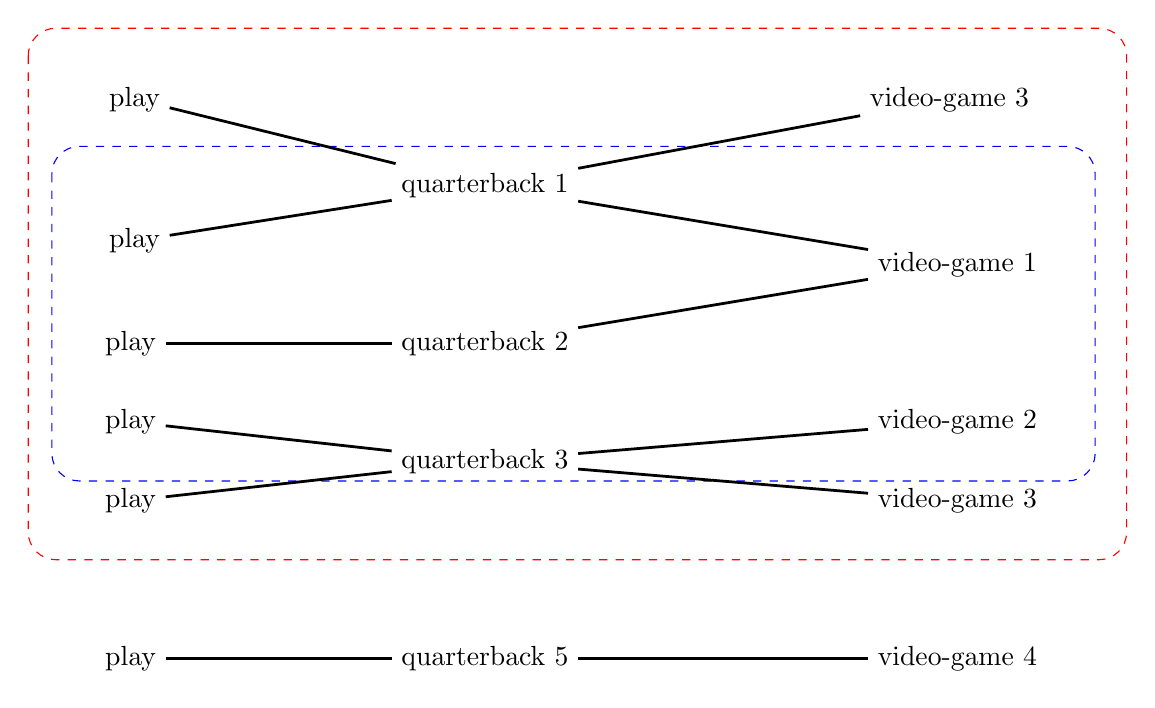
\begin{tikzpicture}[scale = \scale]
\node (v1) at (5.5,1.5) {video-game 1};
\node (v2) at (-0.5,2.5) {quarterback 1};
\node (v4) at (-0.5,0.5) {quarterback 2};
\node (v5) at (5.5,-0.5) {video-game 2};
\node (v6) at (-0.5,-1) {quarterback 3};
\node (v7) at (5.4,3.6) {video-game 3};

\node (v3) at (-4.95,1.8) {play};
\node (v10) at (-5,0.5) {play};
\node (v11) at (-5,-0.5) {play};
\node (v12) at (-4.95,3.6) {play};

\draw [line width = 1pt] (v1) edge (v2);
\draw [line width = 1pt] (v2) edge (v3);
\draw [line width = 1pt] (v1) edge (v4);

\draw [line width = 1pt] (v5) edge (v6);

\draw [line width = 1pt] (v4) edge (v10);
\draw [line width = 1pt] (v6) edge (v11);

\node (v14) at (5.5,-3.5) {video-game 4};
\node (v13) at (-0.5,-3.5) {quarterback 5};
\node (v9) at (-5,-3.5) {play};
\draw [line width = 1pt] (v9) edge (v13);
\draw [line width = 1pt] (v14) edge (v13);
\draw [rounded corners = 10pt, dashed, blue] (-6,3) rectangle (7.25,-1.25);



\node (v15) at (-5,-1.5) {play};
\node (v16) at (5.5,-1.5) {video-game 3};
\draw [line width = 1pt] (v15) edge (v6);
\draw [line width = 1pt] (v6) edge (v16);
\draw [line width = 1pt] (v12) edge (v2);

\draw [line width = 1pt] (v7) edge (v2);
\draw [rounded corners = 10pt, dashed, red] (-6.3,4.5) rectangle (7.65,-2.25);
\end{tikzpicture}

\xe
%
The sentence in \clastxb is made true by the actions of the video-games in the blue dashed frame. However, the blue dashed frame is not true of \clastxa because less than four video-games did the teaching. It is not made true by the red dashed frame either because although four video-games did teach exactly three quarterbacks, they taught them more than one play. This reading serves a particular purpose within Schein's theory but it is useful to think about it from other theories as well. For instance, an event-less operator-based approach would predict that the sentence is true:

\pex
\a{}
[four video games]  [three quarterback] **\textsubscript{At} [a play]
\a \textbf{Predicted truth-conditions:} \\
There are four video-games $X$, three quarterbacks $Y$\\
every one of $X$ taught one of $Y$ a play\\
every one of $Y$ was taught a play by one of $X$
\xe
%
The singular indefinite \emph{a play} is key in generating the reading here. Taking the almost equivalent \quo{one or more plays} yields truth according to my own intuitions:

\ex
Four video-games taught exactly three quarterback one or more plays.
\xe
%
Returning to our local concerns, Schein envisions two logical formulas for the mysterious reading. One that would make use of existential quantification twice and the other just once, conforming to the condition we are trying to evidence.

\pex
\a 
$\exists X\in \text{three-video-games}, \ag({\color{red!80!black}\textsf{pro}_{78}}) = X \wedge $\\
$[\textsf{Exactly 2 } Y\in \text{quarterbacks}, \forall y \in Y, \iota E: \thm(E) = y \wedge \text{teach}(E),$\\
$\exists Z\in \text{two-plays}, \goal({\color{red!80!black} E}) = Z \wedge \text{teach}({\color{red!80!black} E})]^{78}$\\
\a 
$\exists X\in \text{three-video-games}, \ag({\color{red!80!black}\textsf{pro}_{78}}) = X \wedge $\\
$[\textsf{Exactly 2 } Y\in \text{quarterbacks}, \forall y \in Y, \iota E: \thm(E) = y \wedge \text{teach}(E), {\color{blue!80!black} \exists E,}$\\
$\exists Z\in \text{two-plays}, \goal({\color{red!80!black} E}) = Z \wedge \text{teach}({\color{red!80!black} E})]^{78}$\\
\xe
%
\clastxb creates problems.The blue existential in \clastxb allows us to nullify the effect of maximality introduced by the preceding $\iota E$. In other words, instead of requiring that \quo{all that the quarterback $y$ was taught was a new play} as in \clastxa, it is now only required that \quo{\underline{part} of what the quarterback was taught was a new play}. Thus the event described by $g(78)$ may contain for each quarterback more than one play. The red dashed frame for instance is a possible value for $g(78)$ and in that event, it is true that 4 video-games taught.



\end{document}
